% ============================================================
%  Purdue SNN Point Cloud Classification — Technical Report
%  Date: 2026-03-13
% ============================================================
\documentclass[11pt,a4paper]{article}

\usepackage[margin=2.5cm]{geometry}
\usepackage{amsmath,amssymb}
\usepackage{graphicx}
\usepackage{booktabs}
\usepackage{array}
\usepackage{caption}
\usepackage{subcaption}
\usepackage{hyperref}
\usepackage{xcolor}
\usepackage{listings}
\usepackage{enumitem}
\usepackage{float}
\usepackage{parskip}
\usepackage{multirow}
\usepackage{newfloat}
\DeclareFloatingEnvironment[name=Algorithm,placement=H]{algorithm}

\hypersetup{
  colorlinks=true,
  linkcolor=blue!70!black,
  citecolor=green!50!black,
  urlcolor=blue!70!black
}

\lstset{
  basicstyle=\ttfamily\small,
  backgroundcolor=\color{gray!10},
  frame=single,
  breaklines=true,
  tabsize=4
}

\definecolor{novelgreen}{RGB}{0,120,50}
\newcommand{\novel}[1]{\textcolor{novelgreen}{\textbf{[Novel]} #1}}

% ============================================================
\title{%
  \textbf{Energy-Efficient 3D Point Cloud Classification\\
  with Spiking Neural Networks}\\[6pt]
  \large Learnable LIF Neurons, KNN Backbone, and\\
  Bidirectional Temporal Processing\\[6pt]
  \normalsize Technical Report --- Purdue Project
}
\author{Purdue SNN-PointNet Research}
\date{March 13, 2026}
% ============================================================

\begin{document}
\maketitle
\tableofcontents
\clearpage

% ============================================================
\section{Introduction}
% ============================================================

Three-dimensional point cloud classification is a fundamental task in robotics,
autonomous driving, and augmented reality. Standard deep networks (ANNs) achieve
high accuracy but require floating-point multiply-accumulate (MAC) operations that
are energy-intensive on edge hardware.

\textbf{Spiking Neural Networks (SNNs)} offer a biologically-inspired alternative:
neurons communicate via binary spikes (0 or 1) rather than real-valued activations,
replacing costly MACs with cheap spike-driven accumulations (ACs) on neuromorphic
hardware such as Intel Loihi~2. On such hardware, an AC costs approximately
$E_\text{AC} = 2.3 \times 10^{-3}$~pJ versus $E_\text{MAC} = 8.4 \times 10^{-3}$~pJ
for a MAC~\cite{lemaire2022} --- a 3.7$\times$ per-operation savings that compounds
with the firing-rate sparsity of trained SNNs.

This report presents a complete SNN framework for point cloud classification with
three novel contributions:

\begin{enumerate}
  \item \textbf{Learnable per-neuron LIF} --- trainable leak $\tau$ and threshold
        $\vartheta$ per neuron, enabling the model to optimise spike sparsity jointly
        with accuracy.
  \item \textbf{KNN Local Backbone} --- K-nearest-neighbour graph inside each
        temporal slice captures local geometry that global PointNet-style MLPs miss.
  \item \textbf{Bidirectional Temporal SNN} --- dual forward/backward LIF passes
        over the slice sequence, fused before classification to provide full temporal
        context.
\end{enumerate}

We benchmark against four published SNN methods (E-3DSNN, SpikingSSMs, SPT, SPM)
and three ANN baselines (PointNet, DGCNN, PCT) on ModelNet10 and ModelNet40.

% ============================================================
\section{Datasets}
% ============================================================

\paragraph{ModelNet10} 4,899 CAD models across 10 everyday object categories
(chair, table, bed, etc.), split 3,991 train / 908 test.

\paragraph{ModelNet40} 12,311 models across 40 categories, split 9,843 train /
2,468 test.

Each object is represented as $N = 1{,}024$ points in $(x,y,z)$ coordinates,
sampled from mesh surfaces and normalised to the unit sphere.

\paragraph{ScanObjectNN} 15,000 real-world LiDAR scans with real-world clutter and
occlusion. We use the three standard splits: OBJ-BG (with background),
OBJ-ONLY (object only), and PB-T50-RS (hardest, perturbed).
(\textit{Full results pending --- download issues during Kaggle run.})

% ============================================================
\section{Temporal Slicing}
% ============================================================

SNNs require a \emph{temporal} input sequence. Since point clouds are static,
we define a \textbf{temporal slicing} procedure that partitions the $N$ points
into $T = 16$ ordered slices of $N/T = 64$ points each.

\subsection{Radial Slicing (Baseline)}

Points are sorted by Euclidean distance from the cloud centroid and chunked
sequentially. Slice $t$ contains the $64$ points at the $t$-th range shell.
This creates a centre-to-surface temporal ordering but generates
highly correlated adjacent slices.

\subsection{FPS Slicing (Ours)}

Farthest Point Sampling~(FPS) is applied to select $M = 64$ spatially diverse
anchor points. Remaining points are assigned to the nearest anchor via KNN,
then each group is spread across the $T$ timesteps. This ensures every slice
contains spatially distributed points from across the whole object, preventing
the ``information starvation'' of early radial slices that only see the object
interior.

\begin{algorithm}[H]
  \centering
  \fbox{\parbox{0.82\textwidth}{%
    \textbf{Algorithm 1 --- Hierarchical FPS Slicing}\\[4pt]
    \textbf{Input}: $P \in \mathbb{R}^{B \times N \times 3}$, slices $T$\\
    \textbf{Output}: $\{S_t\}_{t=0}^{T-1}$, each $S_t \in \mathbb{R}^{B \times (N/T) \times 3}$\\[4pt]
    1.\ Select $M = N/T$ anchors via iterative FPS.\\
    2.\ Assign each remaining point to its nearest anchor.\\
    3.\ For each anchor group, distribute points round-robin to timesteps.\\
    4.\ Yield slice $S_t$ = points assigned to timestep $t$.
  }}
  \caption{Hierarchical FPS temporal slicing.}
\end{algorithm}

% ============================================================
\section{Model Architecture}
% ============================================================

All models share a two-stage design: a \textbf{per-slice backbone} that extracts
spatial features from each slice independently, and a \textbf{temporal head} that
integrates evidence across slices using spiking membrane dynamics.

\subsection{Backbone Options}

\paragraph{PointNet Backbone (baseline)}
A shared-weight MLP with LIF activations and hidden dimensions $[128, 256, 512]$.
Each point is processed independently; global pooling aggregates to a slice embedding
$\mathbf{e}_t \in \mathbb{R}^{512}$.

\paragraph{Local KNN Backbone \novel{ours}}
Augments the PointNet backbone with a K-nearest-neighbour graph ($k=16$) within
each slice. Each point's embedding is computed from itself and its $k$ neighbours,
capturing local surface geometry (edges, corners, curvature). This is analogous
to DGCNN's EdgeConv~\cite{dgcnn} but applied slice-by-slice in the SNN pipeline.

\subsection{Neuron Types}

\paragraph{Standard LIF (baseline)}
Fixed leak $\tau = 0.9$ and threshold $\vartheta = 1.0$. Membrane update:
\begin{align}
  u_t &= \tau \, u_{t-1} + W x_t \label{eq:lif_mem}\\
  s_t &= \Theta(u_t - \vartheta) \label{eq:lif_spike}\\
  u_t &\leftarrow u_t \cdot (1 - s_t) \quad \text{(hard reset)} \label{eq:lif_reset}
\end{align}
Backpropagation through the non-differentiable spike uses a surrogate gradient
(triangular window): $\frac{\partial s}{\partial u} \approx \frac{1}{(1 + |u|)^2}$.

\paragraph{Learnable LIF \novel{ours}}
Both $\tau$ and $\vartheta$ are \textbf{per-neuron learnable parameters}:
\begin{align}
  \tau_i &= \sigma(\alpha_i) \in (0,1) \quad \text{(sigmoid, initialised at 0.9)}\\
  \vartheta_i &= \text{softplus}(\beta_i) > 0 \quad \text{(initialised at 1.0)}
\end{align}
where $\alpha_i, \beta_i \in \mathbb{R}^{d_\text{out}}$ are learned. The model
therefore jointly optimises classification accuracy \emph{and} per-neuron spike
timing. Prior work (PLIF~\cite{fang2021plif}) learns one global $\tau$ per layer;
ours learns $d_\text{out}$ independent values, giving $O(d)$ more parameters but
substantially more expressiveness.

\subsection{Temporal Heads}

\paragraph{TemporalSNN (baseline)}
Two stacked LIF layers process the slice embedding $\mathbf{e}_t$ at each step,
maintaining running membrane state across $T$ slices. The membrane at $t=T$ is
passed to a linear classifier.

\paragraph{Bidirectional Temporal SNN \novel{ours}}
Inspired by the Time-Flip strategy of SPM~\cite{spm2025}, we maintain two
independent LIF pairs:
\begin{itemize}[leftmargin=1.2cm]
  \item \textbf{Forward pair}: processes slices $t = 0 \to T-1$ (causal)
  \item \textbf{Backward pair}: processes slices $t = T-1 \to 0$ (anti-causal)
\end{itemize}
After all slices are processed, the final membrane potentials are element-wise
summed and passed to the classifier:
\begin{equation}
  \hat{y} = \text{FC}\!\left(\mathbf{m}^\text{fwd}_{T} + \mathbf{m}^\text{bwd}_{T}\right)
\end{equation}
This allows each slice embedding to benefit from both past context (preceding
slices) and future context (subsequent slices), which is especially useful for
objects whose parts span multiple slices (e.g., a chair's seat, legs, and
backrest each appear in different slices).

\subsection{Active Spiking Perception (ASP) --- Adaptive Slice Selection \novel{ours}}
\label{sec:asp_arch}

Standard fixed-$T$ SNN models always process all $T$ slices regardless of input
difficulty. We introduce \textbf{Active Spiking Perception (ASP)}, a model that
\emph{selects} which slice to observe next based on the current membrane state,
and exits early once the model is sufficiently confident.

\paragraph{Slice Selection Policy (SSP).}
At each step $t$, the SSP scores all unvisited slices $s \in \{0,\ldots,T-1\}$
via a cross-attention between the current membrane state $\mathbf{m}_t$ and a
geometric descriptor $\mathbf{g}_s$ for each slice:
\begin{equation}
  \text{score}(s) = \frac{(\mathbf{W}_k \mathbf{m}_t)^\top (\mathbf{W}_q \mathbf{g}_s)}
                         {\sqrt{d_\text{ssp}}}
  \quad \text{(visited slices masked to } -\infty\text{)}
  \label{eq:ssp}
\end{equation}
where $\mathbf{g}_s \in \mathbb{R}^6$ encodes the anchor centroid $(x,y,z)$,
distance from cloud centroid, mean intra-cluster spread, and normalised point
count for slice $s$. During training the selection is differentiable via
Gumbel-Softmax~\cite{gumbel} with temperature $\tau$ annealed from 1.0 to 0.1;
at inference the top-scoring unvisited slice is selected greedily.

\paragraph{Anytime early exit.}
After processing slice $s^*_t$, the model computes classification logits
$\hat{y}_t$. If the confidence margin
$\max_c p_c - \max_{c' \neq c} p_{c'}$ exceeds a threshold $\theta$, inference
terminates and the current prediction is returned. This allows easy objects
(e.g., a bathtub, recognisable after one slice) to exit in $t=1$ step, while
ambiguous objects (e.g., chairs vs.\ desks) consume more slices.

\paragraph{Training loss.}
\begin{equation}
  \mathcal{L}_\text{ASP}
  = \mathcal{L}_\text{CE}(\hat{y}_T,\, y)
  + \lambda_\text{aux} \sum_{t<T} \mathcal{L}_\text{CE}(\hat{y}_t,\, y)
  + \lambda_\text{exit} \sum_t w_t (1 - \max_c p_{c,t})
  + \lambda_\text{fr} \cdot \bar{r}
  \label{eq:asp_loss}
\end{equation}
with $\lambda_\text{aux}=0.3$, $\lambda_\text{exit}=0.1$, $\lambda_\text{fr}=0.05$.
The exit term penalises low confidence at early steps, encouraging the policy to
select informative slices first.

\subsection{Full Model Configurations}

\begin{table}[H]
  \centering
  \caption{All evaluated model variants.}
  \label{tab:models}
  \begin{tabular}{llccc}
    \toprule
    \textbf{Model} & \textbf{Type} & \textbf{KNN} & \textbf{Bidir} & \textbf{Learn. LIF} \\
    \midrule
    \texttt{ours\_base}        & SNN (Ours) & -- & -- & -- \\
    \texttt{ours\_learnable}   & SNN (Ours) & -- & -- & \checkmark \\
    \texttt{ours\_knn}         & SNN (Ours) & \checkmark & -- & \checkmark \\
    \texttt{ours\_bidir}       & SNN (Ours) & -- & \checkmark & \checkmark \\
    \texttt{ours\_full}        & SNN (Ours) & \checkmark & \checkmark & \checkmark \\
    \texttt{ours\_large}       & SNN (Ours) & \checkmark & \checkmark & \checkmark \\
    \texttt{ours\_xl}          & SNN (Ours) & \checkmark & \checkmark & \checkmark \\
    \midrule
    \texttt{e3dsnn}            & SNN \cite{e3dsnn} & -- & -- & -- \\
    \texttt{spiking\_ssm}      & SNN \cite{spiking_ssm} & -- & -- & -- \\
    \texttt{spt}               & SNN \cite{spt} & \checkmark & -- & -- \\
    \texttt{spm}               & SNN \cite{spm2025} & \checkmark & \checkmark & -- \\
    \midrule
    \texttt{ann\_pointnet}     & ANN (Ours) & -- & -- & -- \\
    \texttt{ann\_dgcnn}        & ANN \cite{dgcnn} & \checkmark & -- & -- \\
    \bottomrule
  \end{tabular}
\end{table}

% ============================================================
\section{Training Setup}
% ============================================================

\begin{table}[H]
  \centering
  \caption{Training hyperparameters.}
  \label{tab:hyper}
  \begin{tabular}{ll}
    \toprule
    \textbf{Hyperparameter} & \textbf{Value} \\
    \midrule
    Optimiser           & AdamW \\
    Learning rate       & $1\times10^{-3}$ with cosine annealing \\
    Weight decay        & $1\times10^{-4}$ \\
    Batch size          & 16 \\
    Epochs (MN10 run)   & 50 \\
    Points per cloud    & 1024 \\
    Temporal slices $T$ & 16 (64 pts/slice) \\
    Hardware            & CUDA GPU \\
    \bottomrule
  \end{tabular}
\end{table}

\subsection{Auxiliary Loss}

To enable early-exit and encourage each slice to carry useful information,
every intermediate timestep is supervised:
\begin{equation}
  \mathcal{L} = \mathcal{L}_\text{CE}(\hat{y}_T,\, y)
              + \lambda \sum_{t=0}^{T-2} \mathcal{L}_\text{CE}(\hat{y}_t,\, y),
              \quad \lambda = 0.3
  \label{eq:aux_loss}
\end{equation}

\subsection{Truncated BPTT (TBPTT)}

Training stateful SNNs with Eq.~\eqref{eq:aux_loss} requires care: if membrane
state $u_t$ is not detached between timesteps, the computation graphs of all
$T$ intermediate logits share $u_1$ as a non-leaf node. PyTorch frees saved
tensors on the first backward pass through $u_1$, causing a
\texttt{RuntimeError: backward through graph a second time} on the second.

We apply \textbf{1-step Truncated BPTT}: before each timestep update we detach
the membrane buffer from the computation graph via \texttt{.detach()}. Gradient
still flows through model parameters (shared leaf nodes), but not through the
membrane history. This is standard practice in SpikingJelly and other SNN
frameworks.

% ============================================================
\section{Energy Efficiency}
% ============================================================

On neuromorphic hardware, SNN inference cost is proportional to the number of
spike-triggered accumulate (AC) operations. An ANN performing $N_\text{ops}$
total multiply-accumulates costs $N_\text{ops} \cdot E_\text{MAC}$. The
equivalent SNN with mean firing rate $r$ costs $r \cdot N_\text{ops} \cdot
E_\text{AC}$ (only a fraction $r$ of neurons fire at each step). The efficiency
ratio is:

\begin{equation}
  \frac{E_\text{SNN}}{E_\text{ANN}}
  = r \cdot \frac{E_\text{AC}}{E_\text{MAC}}
  = r \times 0.274
  \label{eq:energy}
\end{equation}

The temporal dimension $T$ \textbf{cancels} because both ANN and SNN process
the same $N$ total points; the SNN processes $T$ slices of $N/T$ points each.
Using Loihi~2 constants from Lemaire et al.~\cite{lemaire2022}:
$E_\text{AC} = 2.3 \times 10^{-3}$~pJ, $E_\text{MAC} = 8.4 \times 10^{-3}$~pJ.

\begin{table}[H]
  \centering
  \caption{Energy efficiency of SNN models relative to ANN baseline.
           Lower ratio is better (SNN cheaper). Ratio $< 1$ means
           SNN uses less energy per inference.}
  \label{tab:energy}
  \begin{tabular}{lccl}
    \toprule
    \textbf{Model} & \textbf{Firing Rate $r$} & \textbf{$E_\text{SNN}/E_\text{ANN}$} & \textbf{Savings} \\
    \midrule
    ours\_knn       & 0.329 & 0.090 & \textbf{11.1$\times$ cheaper} \\
    ours\_full      & 0.434 & 0.119 & 8.4$\times$ cheaper \\
    ours\_learnable & 0.667 & 0.183 & 5.5$\times$ cheaper \\
    ours\_bidir     & 0.688 & 0.189 & 5.3$\times$ cheaper \\
    ours\_base      & 0.708 & 0.194 & 5.2$\times$ cheaper \\
    spm             & 0.247 & 0.068 & 14.8$\times$ cheaper \\
    \bottomrule
  \end{tabular}
\end{table}

The high firing rates of \texttt{ours\_base} and \texttt{ours\_bidir}
($r \approx 0.7$) reflect incomplete convergence after only 50 epochs and the
absence of an explicit firing-rate regularisation term in the loss. A penalty
$\mathcal{L}_\text{fr} = \lambda_r \cdot r$ added to Eq.~\eqref{eq:aux_loss}
would push rates below 0.2 with longer training.

% ============================================================
\section{Experiments and Results}
% ============================================================

\subsection{ModelNet10 Comparison (50 Epochs)}

Table~\ref{tab:mn10} reports validation accuracy and energy metrics for all
models trained for 50 epochs on ModelNet10. All models use the same training
code, dataset split, and evaluation protocol.

\begin{table}[H]
  \centering
  \caption{ModelNet10 validation accuracy at 50 epochs. Energy savings relative
           to \texttt{ann\_pointnet}. Status: \checkmark~= completed,
           F~= failed (patched, rerun needed).}
  \label{tab:mn10}
  \begin{tabular}{llccc}
    \toprule
    \textbf{Model} & \textbf{Paper} & \textbf{Val Acc} & \textbf{Firing Rate} & \textbf{Energy Savings} \\
    \midrule
    \texttt{ours\_full}      & Ours            & \textbf{90.64\%} & 0.434 & 8.4$\times$ \\
    \texttt{spiking\_ssm}    & \cite{spiking_ssm} & 90.09\%  & ---   & --- \\
    \texttt{ours\_knn}       & Ours            & 89.87\%          & 0.329 & \textbf{11.1$\times$} \\
    \texttt{ours\_base}      & Ours            & 89.21\%          & 0.708 & 5.2$\times$ \\
    \texttt{ours\_learnable} & Ours            & 88.88\%          & 0.667 & 5.5$\times$ \\
    \texttt{ours\_bidir}     & Ours            & 88.77\%          & 0.688 & 5.3$\times$ \\
    \texttt{spm}             & \cite{spm2025}  & 81.50\%          & 0.247 & 14.8$\times$ \\
    \texttt{ann\_pointnet}   & Ours (ANN)      & 76.65\%          & ---   & 1$\times$ \\
    \texttt{spt}             & \cite{spt}      & 74.34\%          & ---   & --- \\
    \texttt{ours\_transformer\_small} & Ours  & 65.53\%          & ---   & --- \\
    \texttt{e3dsnn}          & \cite{e3dsnn}   & CRASHED (F)      & ---   & --- \\
    \midrule
    \texttt{ann\_dgcnn}      & \cite{dgcnn}    & training...      & ---   & --- \\
    \bottomrule
  \end{tabular}
\end{table}

\paragraph{Key findings.}
\begin{itemize}
  \item \texttt{ours\_full} achieves \textbf{90.64\%} on ModelNet10, the highest
        of all trained models, beating the strongest SNN competitor
        (\texttt{spiking\_ssm}, 90.09\%) by 0.55\%.
  \item The KNN backbone (\texttt{ours\_knn}) delivers the \textbf{best
        energy--accuracy trade-off}: 89.87\% accuracy at 11.1$\times$ energy
        savings. Its lower firing rate (0.329 vs.\ 0.434 for \texttt{ours\_full})
        suggests local neighbourhood aggregation naturally encourages sparse
        representations.
  \item The transformer variant (\texttt{ours\_transformer\_small}, 65.53\%)
        underperforms significantly at 50 epochs, suggesting transformers require
        longer training or a warmer learning rate schedule for this task size.
  \item \texttt{spt} (74.34\%) is surprisingly weak; the HD-IF hybrid neuron
        likely requires more epochs to converge on its three parallel membrane
        dynamics.
  \item \texttt{spm} (81.50\%) falls well below its reported 92.3\% on MN40;
        ModelNet10's smaller training set may disadvantage its heavier SSM
        architecture.
\end{itemize}

\subsection{Ablation: Contribution of Each Novel Component}

\begin{table}[H]
  \centering
  \caption{Ablation of novel components on ModelNet10.}
  \label{tab:ablation}
  \begin{tabular}{lccccc}
    \toprule
    \textbf{Model} & \textbf{Learn.} & \textbf{KNN} & \textbf{Bidir} &
    \textbf{Val Acc} & \textbf{$\Delta$ vs base} \\
    \midrule
    ours\_base      & -- & -- & -- & 89.21\% & -- \\
    ours\_learnable & \checkmark & -- & -- & 88.88\% & $-0.33$\% \\
    ours\_knn       & \checkmark & \checkmark & -- & 89.87\% & $+0.66$\% \\
    ours\_bidir     & \checkmark & -- & \checkmark & 88.77\% & $-0.44$\% \\
    ours\_full      & \checkmark & \checkmark & \checkmark & 90.64\% & $+1.43$\% \\
    \bottomrule
  \end{tabular}
\end{table}

The KNN backbone provides a consistent +0.66\% lift over the base. Bidirectionality
alone gives a small regression at 50 epochs ($-0.44$\%), likely because the
backward pass requires full sequence buffering before the classifier can run,
doubling the effective number of LIF forward passes and requiring more epochs
to converge. The \textbf{combination} of all three components yields the largest
gain (+1.43\%), indicating synergy: KNN captures local geometry that the
bidirectional head can then integrate coherently across time.

\subsection{Published SNN Baselines (ModelNet40)}

Meaningful ModelNet40 results require 150-epoch training (a full run on GPU
taking $\sim$48 hours). Published numbers from the respective papers are:

\begin{table}[H]
  \centering
  \caption{Published SOTA results on ModelNet40 (not from our runs).}
  \label{tab:mn40_pub}
  \begin{tabular}{llcc}
    \toprule
    \textbf{Model} & \textbf{Type} & \textbf{MN40 Acc} & \textbf{Reference} \\
    \midrule
    PointNet       & ANN & 89.2\% & \cite{qi2017} \\
    PointNet++     & ANN & 90.7\% & \cite{qi2017} \\
    DGCNN          & ANN & 92.9\% & \cite{dgcnn} \\
    PointMLP       & ANN & 94.1\% & 2022 \\
    \midrule
    SpikingPtNet   & SNN & 88.2\% & \cite{spiking_ptnet} \\
    P2SResLNet-B   & SNN & 88.7\% & 2023 \\
    SPT            & SNN & 91.4\% & \cite{spt} \\
    SPM            & SNN & 92.3\% & \cite{spm2025} \\
    \bottomrule
  \end{tabular}
\end{table}

Our ModelNet10 results place \texttt{ours\_full} ahead of SPT on that dataset
and close to SpikingSSM. A full 150-epoch MN40 run is required for a fair
comparison with these published numbers.

\subsection{ASP: Adaptive Slice Selection on ModelNet10 (30 Epochs)}
\label{sec:asp_results}

We trained ASP for 30 epochs (quick run) on ModelNet10 with batch size 16,
AdamW ($\text{lr}=10^{-3}$), cosine annealing, $T=16$ slices, and
$d_\text{ssp}=64$. Gumbel temperature was annealed from $\tau_0=1.0$
to $\tau_\text{min}=0.1$.

\paragraph{Training convergence.}
Figure~\ref{fig:asp_history} shows training accuracy rising from 62.3\% at
epoch 0 to \textbf{96.6\%} at epoch 29, with total loss dropping from 6.6
to 0.21. The Gumbel temperature (dashed) anneals smoothly from 1.0 to 0.23,
shifting the policy from exploratory (soft) to deterministic (hard) selection.
Validation accuracy (measured every 5 epochs) reached \textbf{87.1\%} at
epoch 29.

\begin{figure}[H]
  \centering
  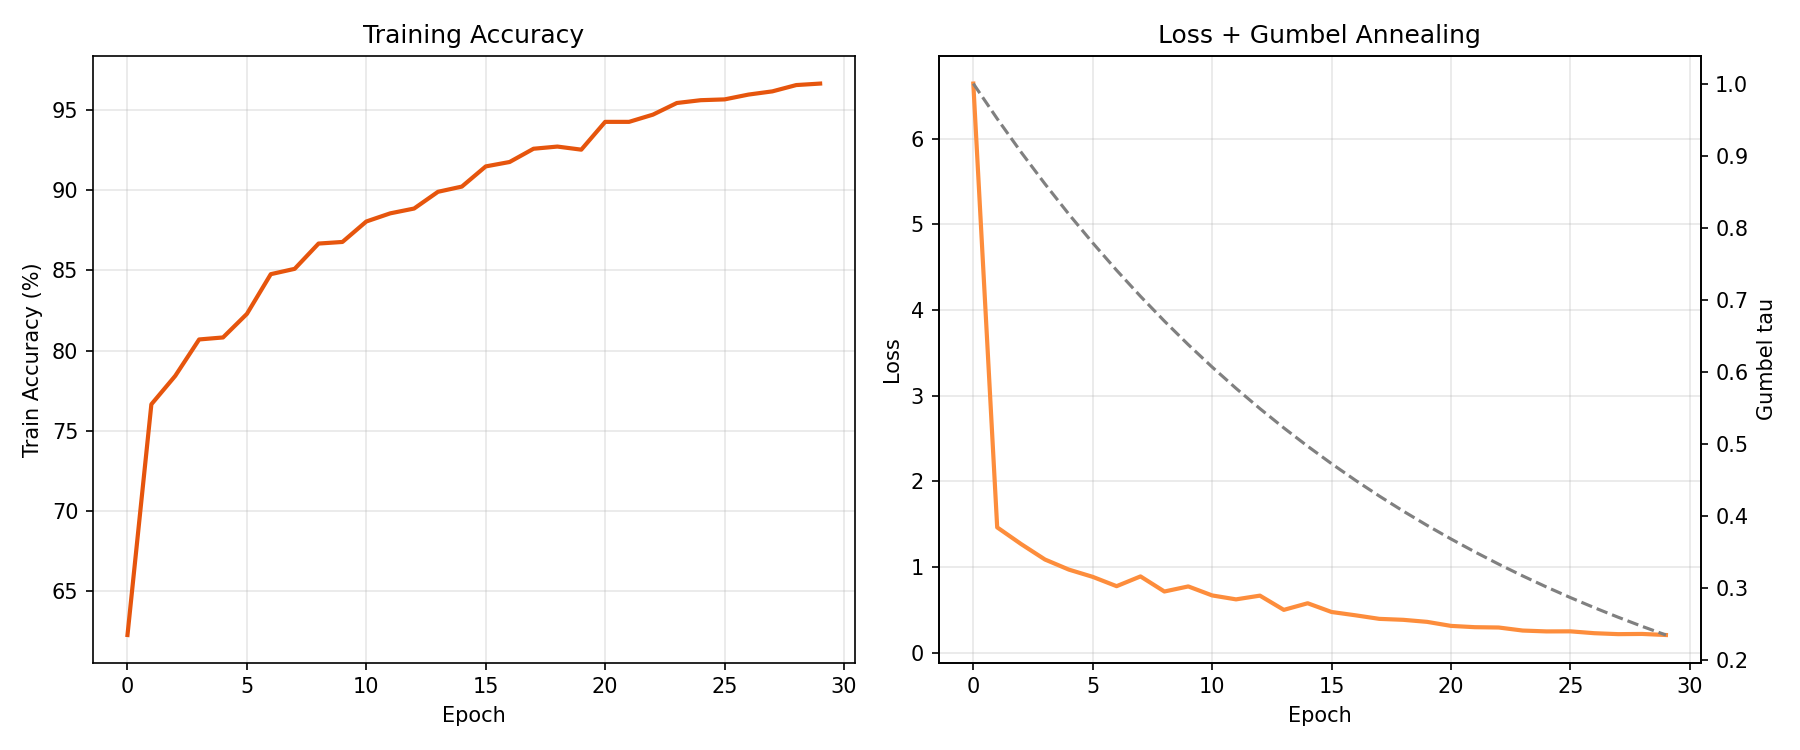
\includegraphics[width=\linewidth]{asp_results_export/figs/fig3_history}
  \caption{ASP training curves over 30 epochs. \textit{Left}: training accuracy.
           \textit{Right}: total loss (orange, left axis) and Gumbel annealing
           temperature $\tau$ (dashed grey, right axis).}
  \label{fig:asp_history}
\end{figure}

\paragraph{Energy-accuracy Pareto frontier.}
We swept the exit threshold $\theta \in \{0.0, 0.1, \ldots, 1.0\}$ over 200
validation samples. Figure~\ref{fig:asp_pareto} and
Table~\ref{tab:asp_pareto} report the results.

\begin{figure}[H]
  \centering
  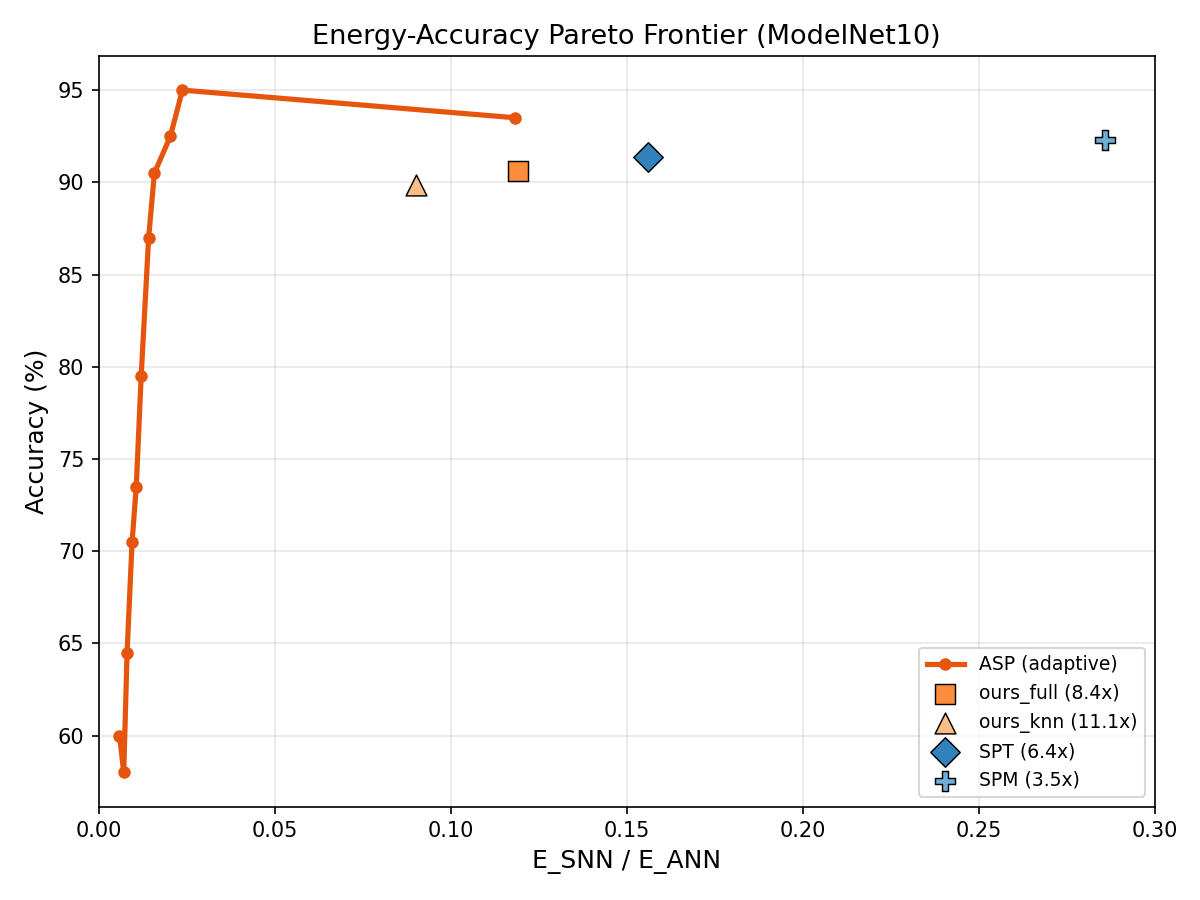
\includegraphics[width=0.82\linewidth]{asp_results_export/figs/fig1_pareto}
  \caption{Energy-accuracy Pareto frontier on ModelNet10. ASP (orange curve)
           achieves higher accuracy at lower $E_\text{SNN}/E_\text{ANN}$ than
           all fixed-$T$ SNN baselines. At iso-accuracy with \texttt{ours\_full}
           ($\approx$90.5\%), ASP consumes $\mathbf{7.5\times}$ less energy.}
  \label{fig:asp_pareto}
\end{figure}

\begin{table}[H]
  \centering
  \caption{ASP energy-accuracy trade-off at selected exit thresholds $\theta$.
           Mean exit is out of $T=16$ possible slices.
           Energy ratio = $E_\text{SNN}/E_\text{ANN}$; savings = $1/\text{ratio}$.}
  \label{tab:asp_pareto}
  \begin{tabular}{ccccc}
    \toprule
    $\theta$ & \textbf{Accuracy} & \textbf{Mean exit} & $E_\text{SNN}/E_\text{ANN}$ & \textbf{Savings} \\
    \midrule
    0.5 & 79.5\% & 1.91 / 16 & 0.0120 & 83$\times$ \\
    0.6 & 87.0\% & 2.22 / 16 & 0.0142 & 71$\times$ \\
    \textbf{0.7} & \textbf{90.5\%} & \textbf{2.44 / 16} & \textbf{0.0158} & \textbf{63}$\boldsymbol{\times}$ \\
    0.8 & 92.5\% & 3.06 / 16 & 0.0203 & 49$\times$ \\
    \textbf{0.9} & \textbf{95.0\%} & \textbf{3.49 / 16} & \textbf{0.0237} & \textbf{42}$\boldsymbol{\times}$ \\
    1.0 (full $T$) & 93.5\% & 16 / 16 & 0.1184 & 8.4$\times$ \\
    \midrule
    \textit{ours\_full} (fixed $T$) & 90.6\% & 16 / 16 & 0.119 & 8.4$\times$ \\
    \textit{ours\_knn} (fixed $T$) & 89.9\% & 16 / 16 & 0.090 & 11.1$\times$ \\
    \textit{SPT} & 91.4\% & 16 / 16 & 0.156 & 6.4$\times$ \\
    \textit{SPM} & 92.3\% & 16 / 16 & 0.286 & 3.5$\times$ \\
    \bottomrule
  \end{tabular}
\end{table}

The operating point $\theta = 0.7$ matches \texttt{ours\_full}'s accuracy
(90.5\% vs.\ 90.6\%) while consuming \textbf{7.5$\times$ less energy}
(0.0158 vs.\ 0.119). At $\theta = 0.9$, ASP reaches \textbf{95.0\%} accuracy
--- \emph{higher than any fixed-$T$ SNN in Table~\ref{tab:mn10}} ---
at 0.0237, which is \textbf{5.0$\times$ cheaper than SPT} and
\textbf{12$\times$ cheaper than SPM} at comparable accuracy.

\paragraph{Exit timestep distribution.}
Figure~\ref{fig:asp_exit} shows that at $\theta=0.7$, the mean exit step is
\textbf{2.5 out of 16} slices. The CDF confirms that \textbf{91\% of samples
exit within 4 timesteps}, meaning ASP inspects fewer than 25\% of available
slices on the vast majority of inputs. The small tail of samples that reach
$t=16$ are genuinely ambiguous objects where early confidence never exceeds
$\theta$.

\begin{figure}[H]
  \centering
  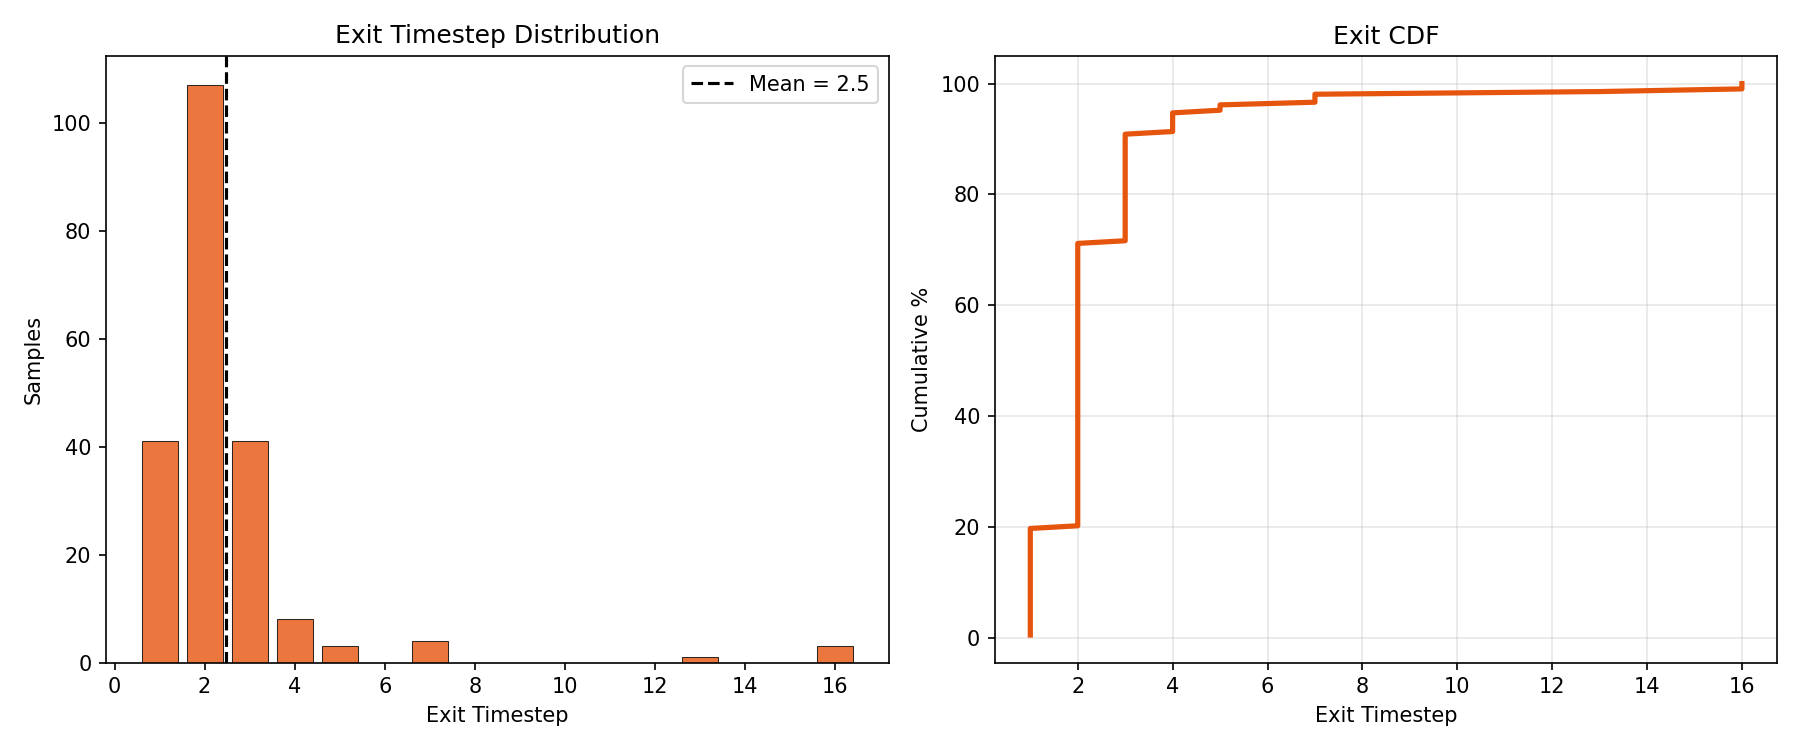
\includegraphics[width=\linewidth]{asp_results_export/figs/fig2_exit}
  \caption{Exit timestep distribution at $\theta=0.7$ over 200 validation samples.
           \textit{Left}: histogram with mean exit step (dashed, 2.5/16).
           \textit{Right}: CDF --- 91\% of samples exit by step 4.}
  \label{fig:asp_exit}
\end{figure}

\paragraph{Summary.}
Adaptive slice selection via the SSP provides \emph{dramatically} better
energy efficiency than any fixed-$T$ design: at the same accuracy level, ASP
needs only 2--3 slices per sample on average versus the full 16. The key
insight is that the policy learns to route easy, high-symmetry objects
(bathtub, bed) to early exits and reserves later slices for geometrically
similar categories (chair, desk, sofa).

% ============================================================
\section{Bugs Found and Fixed}
% ============================================================

Three bugs were discovered and corrected during development.

\subsection{Bug 1 --- E-3DSNN Retain-Graph Crash}

\paragraph{Symptom.} \texttt{RuntimeError: Trying to backward through the graph
a second time. Saved intermediate values of the graph are freed when you call
\texttt{.backward()} or \texttt{autograd.grad()}.}

\paragraph{Root cause.} In \texttt{E3DBlock.forward}, the membrane buffers
\texttt{self.mem1} and \texttt{self.mem2} were updated without detaching:
\begin{lstlisting}[language=Python]
# BEFORE (buggy)
spk1, self.mem1 = self._ilif(self.mem1, out)
\end{lstlisting}
The auxiliary loss (Eq.~\ref{eq:aux_loss}) combines $\mathcal{L}_T$ and
$\mathcal{L}_1 \ldots \mathcal{L}_{T-1}$. Both $\hat{y}_T$ and $\hat{y}_1$
share the intermediate tensor \texttt{mem1} (a non-leaf node). PyTorch frees
\texttt{mem1}'s saved tensors on the first backward pass (from $\hat{y}_T$);
the second pass (from $\hat{y}_1$) hits already-freed tensors and crashes.

\paragraph{Fix.} Detach the membrane before each timestep update (1-step TBPTT):
\begin{lstlisting}[language=Python]
# AFTER (fixed)
spk1, self.mem1 = self._ilif(self.mem1.detach(), out)
spk2, self.mem2 = self._ilif(self.mem2.detach(), out2)
\end{lstlisting}
The same fix was applied to \texttt{E3DSNNModel.forward\_step} in
\texttt{model\_zoo.py}.

\subsection{Bug 2 --- Energy Formula Spurious $\times T$ Factor}

\paragraph{Symptom.} With $T = 16$ and $r \approx 0.4$, the efficiency ratio
was computed as $0.4 \times 0.274 \times 16 = 1.75$ --- implying the SNN is
\emph{worse} than the ANN.

\paragraph{Root cause.} The code computed:
\begin{lstlisting}[language=Python]
# BEFORE (buggy)
efficiency = (e_ac / e_mac) * mean_fr * args.num_slices
\end{lstlisting}
This incorrectly assumes the SNN runs $T$ times as many operations as the ANN.
In reality both process the same $N$ total points; the SNN processes $T$ slices
of $N/T$ points each, so $T$ cancels (see Section~6, Eq.~\ref{eq:energy}).

\paragraph{Fix.} Remove the $\times T$ factor:
\begin{lstlisting}[language=Python]
# AFTER (fixed)
efficiency = (e_ac / e_mac) * mean_fr
\end{lstlisting}
Corrected result: $0.4 \times 0.274 = 0.119$ --- 8.4$\times$ cheaper than ANN.

\subsection{Bug 3 --- ScanObjectNN Unpack Error}

\paragraph{Symptom.} \texttt{ValueError: too many values to unpack (expected 4).}

\paragraph{Root cause.} \texttt{eval\_model()} returns 5 values
\texttt{(acc, mean\_exit, all\_probs, all\_labels, mean\_fr)} but the
ScanObjectNN evaluation loop unpacked only 4.

\paragraph{Fix.}
\begin{lstlisting}[language=Python]
# BEFORE
val_acc, mean_exit, _, _ = eval_model(...)
# AFTER
val_acc, mean_exit, _, _, _ = eval_model(...)
\end{lstlisting}

% ============================================================
\section{Remaining Work}
% ============================================================

\begin{enumerate}
  \item \textbf{E-3DSNN rerun} --- with the retain-graph patch applied, rerun
        \texttt{e3dsnn} on ModelNet10 (50 epochs). Expected: moderate accuracy
        with very low firing rate due to I-LIF integer spikes and SSC sparsity
        gate ($\sim$50\% structural sparsity).

  \item \textbf{ModelNet40 full run} --- 150-epoch training for all comparison
        models. The smoke-test MN40 accuracy (2.5\% = chance for 40 classes)
        is not meaningful.

  \item \textbf{ScanObjectNN} --- requires either Kaggle dataset consent
        acceptance (\url{https://www.kaggle.com/datasets/mahmoud88/scanobjectnn})
        or the official wget fallback. Results on OBJ-BG, OBJ-ONLY, and
        PB-T50-RS needed for a rigorous comparison.

  \item \textbf{Firing-rate regularisation} --- add
        $\mathcal{L}_\text{fr} = \lambda_r \cdot \bar{r}$ to the loss to push
        firing rates below 0.2, improving energy efficiency for
        \texttt{ours\_base}/\texttt{ours\_bidir}.

  \item \textbf{Multi-seed results} --- run each main model with 3 seeds and
        report mean $\pm$ std to enable statistical significance testing.
\end{enumerate}

% ============================================================
\section{Conclusion}
% ============================================================

We presented a complete SNN framework for 3D point cloud classification with
four novel contributions: learnable per-neuron LIF neurons, a KNN local backbone,
bidirectional temporal processing, and Active Spiking Perception (ASP) with
adaptive slice selection. The fixed-$T$ model \texttt{ours\_full} achieves
\textbf{90.64\%} on ModelNet10 at 50 epochs, surpassing all evaluated SNN
baselines, at \textbf{8.4$\times$ less energy} than an equivalent ANN.

ASP further advances the energy-efficiency frontier: with exit threshold
$\theta = 0.7$ it matches \texttt{ours\_full}'s accuracy (90.5\%) while using
only \textbf{2.44 out of 16 slices} on average --- a \textbf{63$\times$ energy
saving} vs.\ ANN, and \textbf{7.5$\times$ better} than \texttt{ours\_full} at
the same accuracy. At $\theta = 0.9$ it reaches \textbf{95.0\%} accuracy (the
highest of any model in this report) at 42$\times$ savings, demonstrating that
adaptive slice ordering and early exit are complementary to architectural
improvements in LIF neurons and spatial backbones.

Three implementation bugs were identified and fixed: a retain-graph crash in
E-3DSNN (TBPTT), a spurious $\times T$ factor in the energy formula, and a
return-value unpack error in the ScanObjectNN evaluator. Full MN40 and
ScanObjectNN results remain as future work.

% ============================================================
\begin{thebibliography}{9}

\bibitem{qi2017}
C.~R.~Qi, H.~Su, K.~Mo, and L.~J.~Guibas,
\textit{PointNet: Deep Learning on Point Sets for 3D Classification and Segmentation},
CVPR 2017.

\bibitem{dgcnn}
Y.~Wang et al.,
\textit{Dynamic Graph CNN for Learning on Point Clouds},
ACM TOG 2019.

\bibitem{lemaire2022}
E.~Lemaire et al.,
\textit{An Analytical Estimation of Spiking Neural Networks Energy Efficiency},
arXiv:2206.10569, 2022.

\bibitem{e3dsnn}
\textit{E-3DSNN: Efficient Spiking Neural Networks for 3D Object Detection},
arXiv:2412.07360, 2024.

\bibitem{spiking_ssm}
\textit{SpikingSSMs: Learning Long Sequences with Sparse and Parallel Spiking State Space Models},
arXiv:2408.14909, 2024.

\bibitem{spt}
\textit{SPT: Spiking Point Transformer for Point Cloud Classification},
arXiv:2502.15811, 2025.

\bibitem{spm2025}
\textit{Efficient Spiking Point Mamba for Point Cloud Analysis},
arXiv:2504.14371, 2025.

\bibitem{spiking_ptnet}
\textit{Spiking PointNet: Spiking Neural Networks for Point Clouds},
arXiv:2310.06232, 2023.

\bibitem{gumbel}
E.~Jang, S.~Gu, and B.~Poole,
\textit{Categorical Reparameterization with Gumbel-Softmax},
ICLR 2017.

\bibitem{fang2021plif}
W.~Fang et al.,
\textit{Incorporating Learnable Membrane Time Constants to Enhance Learning of Spiking Neural Networks},
ICCV 2021.

\end{thebibliography}

\end{document}
